\chapter{\Large Iteración II: “Información contextual y envió de alertas de seguridad”}
\begin{section}{Verificación del requerimiento funcional 2: Recolección de información contextual}
    Con el objetivo de recibir y procesar información contextual de los activos que se ven afectados durante un incidente, fue necesario configurar el servidor Master de Security Onion, con otros servicios que permitieran recibir información diferente de la provista por los sensores. Esta información refleja el estado de los servicios en un servidor, su conexión a la red, parámetros de uso de hardware como el nivel de ocupación de disco, temperatura, uso de la memoria RAM, los logs referidos al procesamiento de las peticiones que recibe un servidor, etc. \par
    Una anomalía en los datos de esta información no es suficiente para confirmar un ataque, pero es útil para indicar que algo puede estar ocurriendo. En el caso de un ataque confirmado, estos datos representan evidencia forense y sirven para enriquecer modelos de amenazas complejas. \par
   
    Se decidió enviar la información contextual disponible mediante Filebeat. Este es un servicio que permite enviar información a Logstash desde múltiples directorios. El proceso comienza cuando el servicio lee línea por línea los archivos de entrada y envía los logs de la misma manera a Logstash. Este los recibe en su puerto 5044 por defecto, posteriormente puede filtrarlos para separar los campos de los logs o bien almacenarlos sin filtrar. \par
    %Al principio enviamos los logs del estado de las aplicaciones de un servidor disponible en la organización, mediante Filebeat, a Logstash y sin un procesamiento posterior. Esto generó que ElastAlert no pudiera identificar información clave para realizar una correlación, como la que se encuentra en los campos de puertos y direcciones IP de origen y destino, estampas de tiempo, tipo de peticiones, etc. \par
    Al principio se envió los logs del estado de las aplicaciones de un servidor disponible en la organización, mediante Filebeat, a Logstash y sin un procesamiento posterior. Esto generó que ElastAlert no pudiera realizar una correlación al no identificar información clave, como la que se encuentra en los campos de puertos y direcciones IP de origen y destino, estampas de tiempo, tipo de peticiones, etc.\par
    Posteriormente se utilizo el plugin grok para filtrar los logs que estaba recibiendo Logstash antes de almacenarlos, de manera que la detección basada en correlaciones fue posible.\par
    Como se observa en la Figura \ref{fig:iter2_despl_dist} y tal como se describió en la sección \ref{subsection:topo_dist}, se realizo el envío de logs mediante Filebeat. Estos logs contenían información de ataques a activos de la organización en el pasado. 
    \begin{figure}[H]
    \centering
        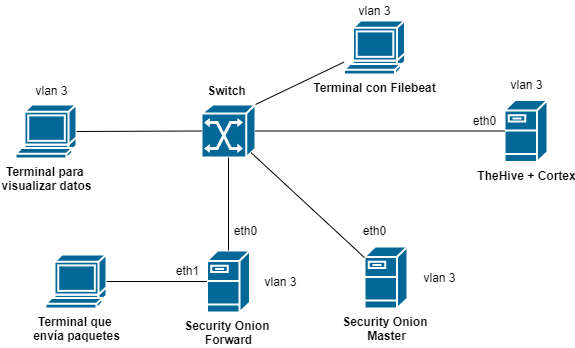
\includegraphics[width=0.7\textwidth]{./iteracion_1_imagenes/figura_33_c_topologia_de_prueba_3.png}
        \caption{Despliegue distribuido de prueba}
        \label{fig:iter2_despl_dist}
    \end{figure}
    \FloatBarrier
    Como se mencionó anteriormente, en primer lugar los logs se almacenaron sin filtrar, lo que ocasionó que no fuese posible realizar algún tipo de correlación con los datos obtenidos. En la Figura \ref{fig:iter2_logs_crudos} se puede observar el almacenamiento de estos registros, con esto queda demostrado el cumplimiento del requerimiento funcional 2.
    %INSERTAR ACA FIGURA 6.2 "LOGS SIN PROCESAR"
    \begin{figure}[H]
    \centering
        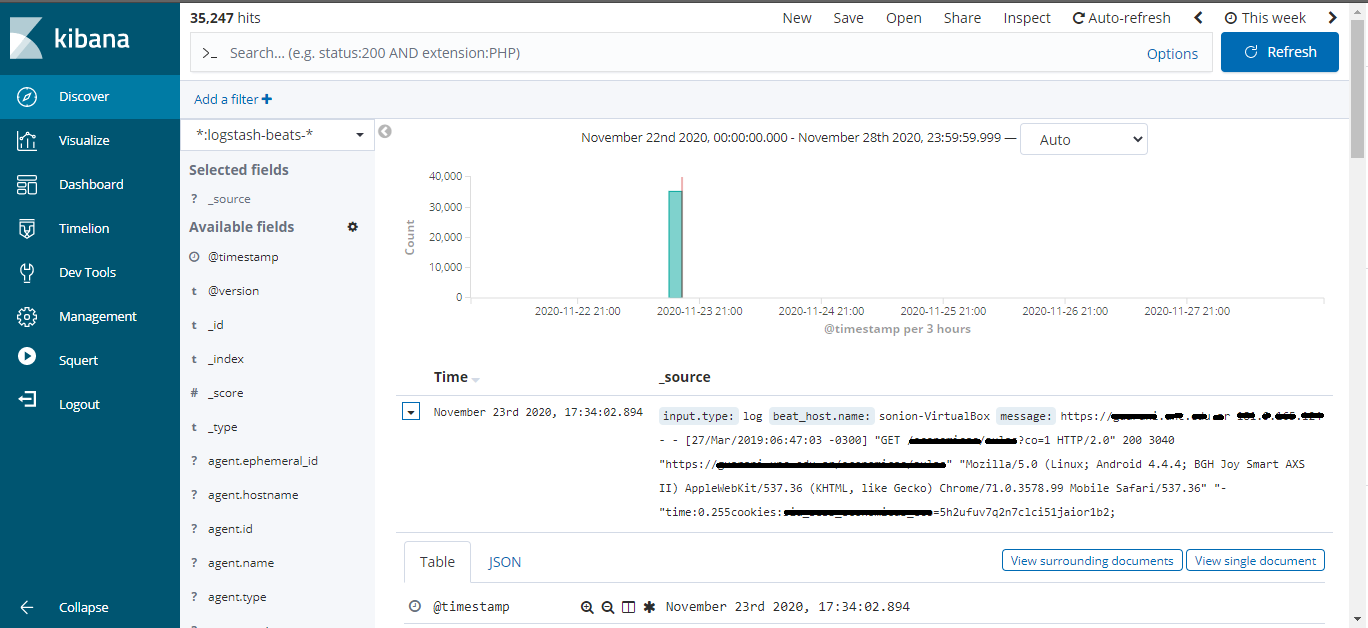
\includegraphics[width=1\textwidth]{./iteracion_2_imagenes/1_kibana_logs_1EDITADA.png}
        \caption{Almacenamiento de logs sin procesar}
        \label{fig:iter2_logs_crudos}
    \end{figure}
    \FloatBarrier
    Posteriormente se repitió la experiencia pero esta vez los logs que se recibían en Logstash eran procesados utilizando grok. Grok es un plugin de Logstash que permite filtrar datos sin ningún tipo de estructura y generar información estructurada capaz de ser consultada.
    Los resultados se pueden ver en la Figura \ref{fig:iter2_logs_filtrados}.\par
    %INSERTAR ACA FIGURA 6.3 "LOGS PROCESADOS"
    \begin{figure}[H]
    \centering
        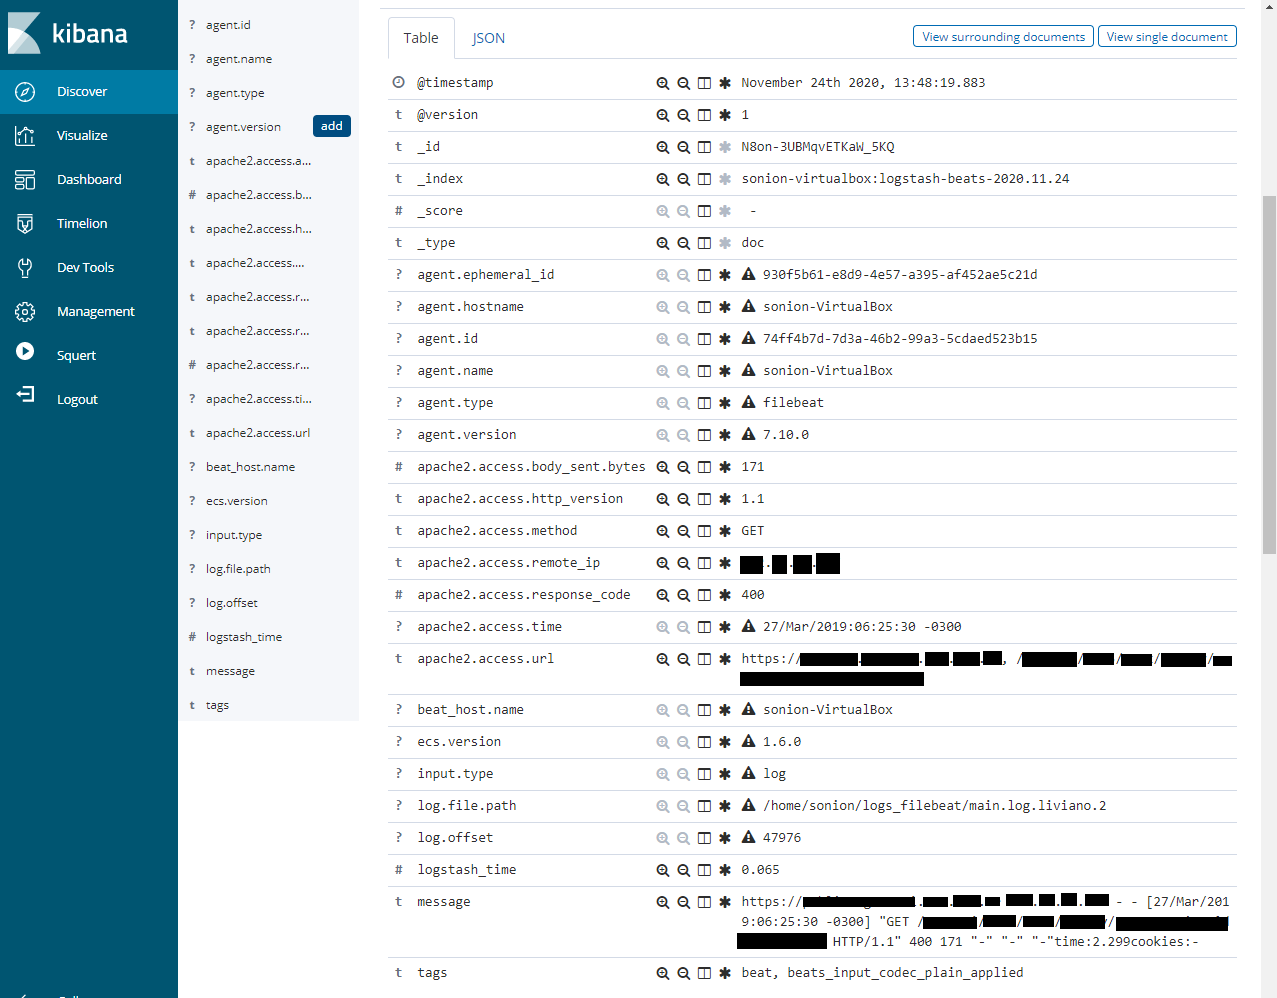
\includegraphics[width=1\textwidth]{./iteracion_2_imagenes/kibana_logs_parseados_2EDITADO.png}
        \caption{Almacenamiento de logs procesados por Logstash}
        \label{fig:iter2_logs_filtrados}
    \end{figure}
    Logstash posee varios filtros para todos los tipos de entradas que soporta. 
    Fue posible editar y administrar estos filtros utilizando archivos de configuración ubicados en la carpeta \textit{/etc/logstash/conf.d.available/}. Para este proyecto se eligió editar el filtro que procesa los datos provenientes de Filebeat, como se indicó anteriormente.\par
    El proceso de creación de este filtro consistió en copiar el archivo de configuración de Filebeat: \textit{9500\_output\_beats\_custom.conf} que se encuentra en el directorio mencionado anteriormente. El archivo fue copiado a la carpeta \textit{/etc/logstash/custom}, donde fue modificado para crear el filtro con Grok. Este fue creado teniendo en cuenta el cuerpo de los mensajes provenientes del archivo de logs analizado, dado que se conocían los campos de interés que contenían los logs y que por lo tanto se deseaba extraer. Una vez finalizada la modificación del archivo, se reinicio el servicio de Logstash y se comprobó que el archivo \textit{logstash.log} para verificar que no hubiera errores.\par
    Es importante mencionar que la información almacenada en Elasticsearch, es consultada constantemente por ElastAlert. Este ultimo componente es el encargado de correlacionar los campos de los logs y enviar notificaciones.

    \end{section}
    
    \begin{section}{Verificación de requerimiento funcional 6 y 4: implementación de un sistema de correlación y envió de alertas de seguridad}
    El envío de alertas de seguridad y la notificación a los responsables de los activos que se ven afectados, fue realizado en este trabajo mediante ElastAlert. Este componente fue seleccionado ya que permite correlacionar la información presente en los campos de logs guardados en elasticsearch, así como enviar notificaciones cuando se produce la detección de incidentes. \par
    ElastAlert es un framework que detecta patrones en los datos consultados a Elasticsearch, como anomalías, picos, etc. Como se mencionó en la sección \ref{seccion4-5}, basa su funcionamiento en dos componentes: reglas y alertas. \par
    Las alertas consisten en mensajes que permiten notificar a un usuario final o a otro sistema, sobre un evento de seguridad que ha ocurrido. Para esta prueba se decidió que las notificaciones fueran enviadas por correo electrónico a una dirección asignada por la organización.\par
    Se escribieron archivos de configuración para cada tipo de evento, de manera tal que las reglas que disparan cada alerta lo hagan según el comportamiento y naturaleza del incidente. En las figuras \ref{fig:iter2_1_codigo} a \ref{fig:iter2_4_codigo} se observa el código desarrollado para el envío de alertas en caso de producirse un reconocimiento y escaneo de puertos. Las figuras corresponden al mismo archivo de configuración, pero cada una muestra una parte del código para facilitar la explicación del mismo.\par
    En la Figura \ref{fig:iter2_1_codigo} se muestra la primer parte del código de configuración de una regla:
    \begin{itemize}
        \item \textit{es\_host}: el nombre del host de la base de datos elasticsearch.
        \item \textit{es\_port}: el número de puerto del host de elasticsearch mediante el cual ElastAlert se contactara con la base de datos.
        \item \textit{name}: nombre de la regla. Debe ser único.
        \item \textit{type}: especifica el tipo de regla. En este caso es del tipo “frecuency”, que determina que esta regla se activará si al menos se produce cierto número de eventos en determinado intervalo de tiempo.
        \item \textit{num\_events}: especifica la cantidad de eventos necesarios para activar este tipo de regla.
        \item \textit{timeframe}: determina el marco temporal necesario para este tipo de reglas. Tiene un sub parámetro que especifica la unidad temporal y la cantidad de estas. En este caso optamos por un marco temporal de un (1) minuto.
    \end{itemize}
    \begin{figure}[H]
    \centering
        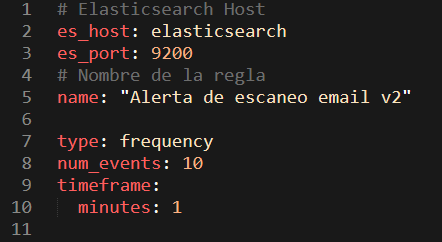
\includegraphics[width=0.7\textwidth]{./iteracion_2_imagenes/3-codigoAlerta-1.png}
        \caption{Primera parte del código de configuración de una regla}
        \label{fig:iter2_1_codigo}
    \end{figure}
    \FloatBarrier
    En la Figura \ref{fig:iter2_2_codigo} se muestran los campos implicados en la consulta a elasticsearch:
    \begin{itemize}
        \item \textit{index}: es el índice a consultar
        \item \textit{use\_strftime\_index}: es una variable booleana que, en el caso de ser verdadera, da formato al índice utilizando “\textit{datetime\_strftime}” para cada consulta. Este último método de Python crea un string representando el tiempo en un formato específico. Se utiliza en el caso de que la consulta realizada incluya varios días, con lo que los índices se concatenan utilizando “;” permitiendo una búsqueda más eficiente.
        \item \textit{filter}: determina los filtros de elasticsearch utilizados para la consulta. Utiliza los subparametros “term”  y “category” para indicar la clave a buscar. En este caso utilizamos “category: scan” para filtrar todos los eventos que pertenezcan a la categoría del reconocimiento de puertos.
        \item \textit{query\_term}: permite agrupar las consultas, en este caso agrupamos las alertas resultantes por direcciones IP de origen y destino, así como todos los eventos que tengan el campo “alert”.
        \item \textit{realert}: ignora las alertas repetidas en un cierto periodo de tiempo. En la práctica esto permitió evitar saturar con notificaciones a los responsables de los activos afectados, ya que el reconocimiento de puertos es un incidente extremadamente común y periódico, produciéndose muchas veces por día.
    \end{itemize}
    \begin{figure}[H]
    \centering
        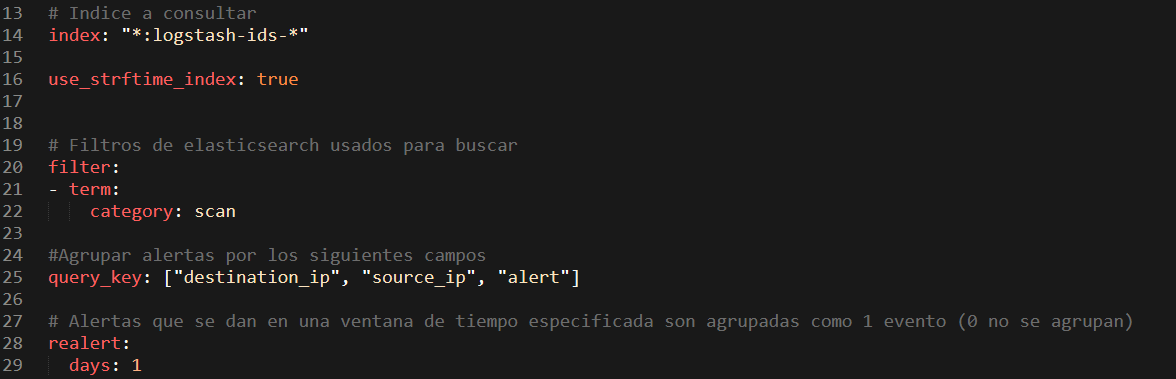
\includegraphics[width=1\textwidth]{./iteracion_2_imagenes/4-codigoAlerta2.png}
        \caption{Segunda parte del código de configuración de una regla}
        \label{fig:iter2_2_codigo}
    \end{figure}
    \FloatBarrier
    En la Figura \ref{fig:iter2_3_codigo} se observan los campos utilizados para armar el cuerpo del mensaje y el asunto:
    \begin{itemize}
        \item \textit{doc\_type}: especifica el tipo de documento a consultar en elasticsearch.
        \item \textit{alert\_subject}: permite personalizar el mensaje de una alerta agregando un pequeño resumen. En este proyecto lo utilizamos en todas las reglas, para que el “asunto” del correo electrónico contenga un mensaje de “Alerta: tipo-de-alerta”. En este caso el argumento ({0}) que figura es el primer campo (tipo de alerta) del objeto JSON que contiene la información del incidente.
        \item \textit{alert\_subject\_args}: contiene el nombre del campo que será utilizado por \textit{alert\_subject}
        \item \textit{alert\_text}: contiene el mensaje de la notificación, se decidió presentar en una lista los parámetros más importantes de los incidentes. Estos incluyen el nombre de la alerta (que también está en el asunto del correo), timestamp indicando la fecha y hora de la detección del incidente, dirección IP de destino, el puerto de destino, dirección IP y puerto de origen, la interfaz del sensor que realizó la detección, información sobre la firma del incidente y un link para verlo en kibana.
        \item \textit{alert\_text\_type}: especifica el formato del texto de la alerta, en este caso optamos por utilizar la sintaxis de formato standard de Python.
        \item \textit{alert\_text\_args}: contiene los nombres de los campos cuyos valores serán utilizados para el contenido del mensaje.
    \end{itemize}
    \begin{figure}[H]
    \centering
        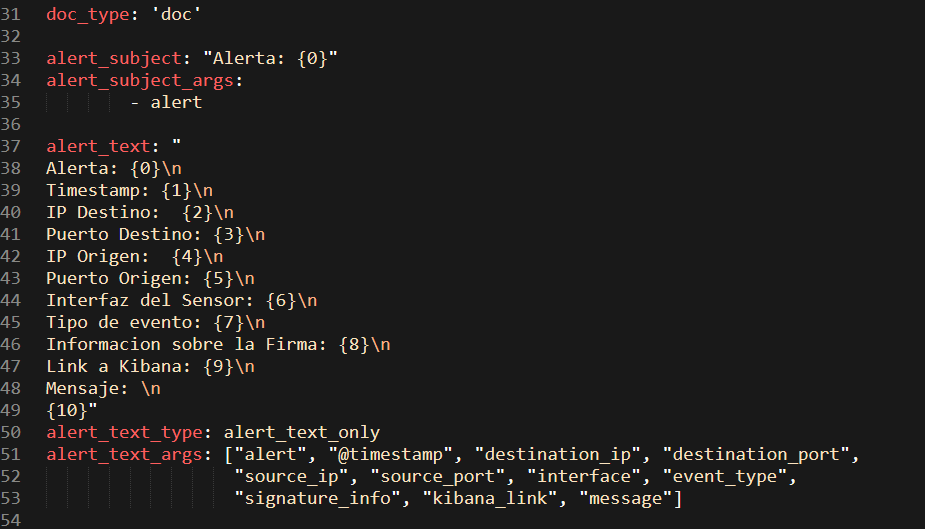
\includegraphics[width=1\textwidth]{./iteracion_2_imagenes/5-codigoAlerta3.png}
        \caption{Tercera parte del código de configuración de una regla}
        \label{fig:iter2_3_codigo}
    \end{figure}
    \FloatBarrier
    En la Figura \ref{fig:iter2_4_codigo} se observan los campos correspondientes al envío de la notificación:
    \begin{itemize}
        \item \textit{alert}: determina el tipo de alerta implementada, es decir, el método de envío. ElastAlert puede enviar mensajes y notificaciones por varios medios que incluyen el correo electrónico, servicios y aplicaciones, como Telegram, JIRA, entre otros. En este proyecto se decidió utilizar el correo electrónico de la organización como medio de notificación de alertas.
        \item \textit{email}: campo que contiene el correo electrónico de destino. Puede ser una dirección o una lista de direcciones de correos.
        \item \textit{from\_addr}: este campo contiene el correo electrónico remitente que ElastAlert utilizará para enviar las notificaciones.
        \item \textit{smtp\_host}: servidor SMTP del correo utilizado para enviar las notificaciones.
        \item \textit{smtp\_port}: puerto utilizado por el servidor SMTP.
        \item \textit{generate\_kibana\_link}: variable booleana que de estar activada genera un tablero temporal de Kibana y un link para acceder a el.
        \item \textit{use\_kibana4\_dashboard}: link hacia un tablero de Kibana (versión 4).
    \end{itemize}
    \begin{figure}[H]
    \centering
        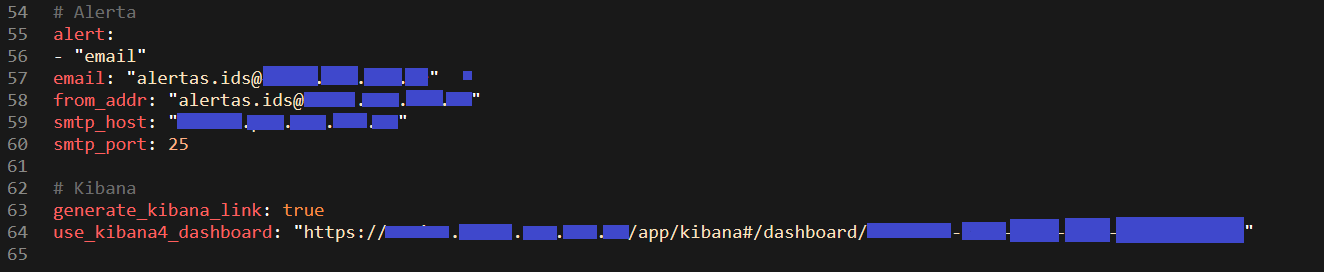
\includegraphics[width=1\textwidth]{./iteracion_2_imagenes/6-codigoAlerta4.png}
        \caption{Cuarta parte del código de configuración de una regla}
        \label{fig:iter2_4_codigo}
    \end{figure}
    \FloatBarrier
    En la Figura \ref{fig:iter2_diagrama_envio_alertas} se observa un diagrama de secuencia del envío de una alerta.
    La secuencia comienza cuando los logs que llegan a Logstash son filtrados y enviados de forma estructurada (JSON) al puerto 9200 de Elastisearch. ElastAlert, por otro lado, realiza consultas periódicas a Elasticsearch. Cuando ElastAlert recibe una respuesta a su petición, procede a analizar los resultados en búsqueda de patrones que se puedan identificar en los logs recibidos. \par
    Independientemente de la coincidencia o no de algún patrón y la eventual notificación de alerta a los correspondientes responsables, ElastAlert vuelve a consultar a Elasticsearch por otros logs y procede a repetir el procedimiento descrito, mientras este activo como servicio.\par 
    \begin{figure}[H]
    \centering
        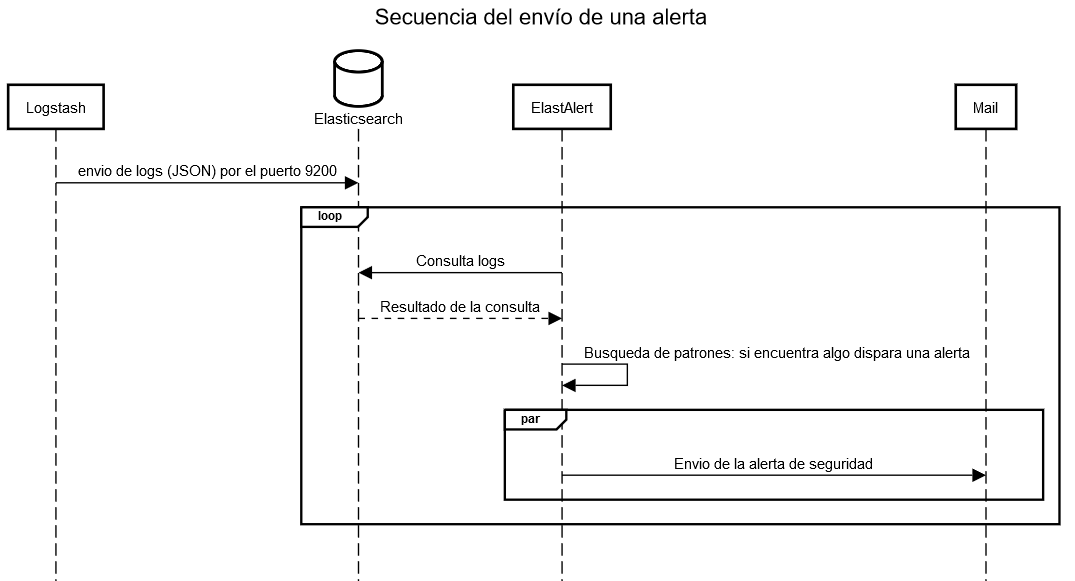
\includegraphics[width=1\textwidth]{./iteracion_2_imagenes/2-diagrama-de-secuencia-envio-alerta.png}
        \caption{Diagrama de secuencia del envío de una alerta}
        \label{fig:iter2_diagrama_envio_alertas}
    \end{figure}
    Los patrones a buscar están definidos en las reglas habilitadas de ElastAlert y si se produce una coincidencia, se procede a enviar una notificación por los medios especificados en las reglas. Como se mencionó anteriormente, para esta prueba el medio elegido fue el correo electrónico de la organización. En la Figura \ref{fig:iter2_notificacion_alertas} se observa el correo electrónico recibido cuando se disparó una alerta sobre un ataque de reconocimiento. Con esto damos por verificado los requerimientos funcionales 4 y 6, dado que para que la notificación haya sido enviada, previamente se tuvo que ejecutar una correlación, como se describió anteriormente.
    \begin{figure}[H]
    \centering
        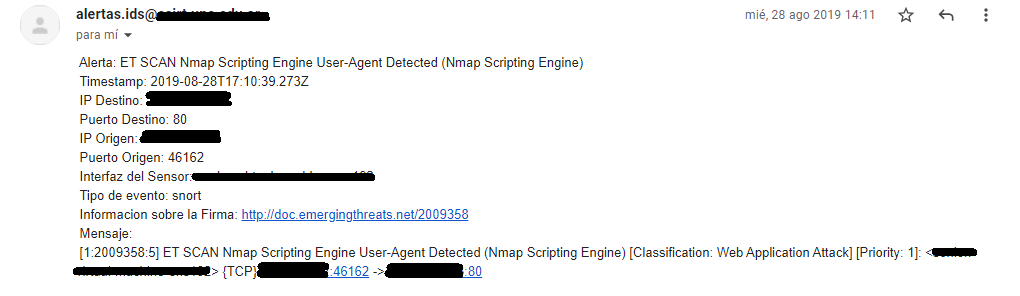
\includegraphics[width=1\textwidth]{./iteracion_2_imagenes/notificacion_alertas_1EDITADO.png}
        \caption{Notificación recibida debido a una alerta por reconocimiento de puertos}
        \label{fig:iter2_notificacion_alertas}
    \end{figure}
    \end{section}
    \begin{section}{Verificación del requerimiento no funcional 3: Escalabilidad de la solución}
    Como se demostró en el capítulo 5, se desarrollaron distintas topologías de red, desde la monolítica hasta las variantes distribuidas. La topología distribuida admite un conjunto de varios nodos Forward y un nodo Master, lo que evidencia la capacidad de escalamiento horizontal de Security Onion. En este proyecto realizamos un despliegue de tres nodos Forward, sin embargo sólo dos nodos estuvieron activos la mayor parte del tiempo.\par
    Dadas las restricciones de hardware con las que se contaba, no fue posible verificar el número máximo de nodos Forward que es posible administrar con un único nodo Master. Sin embargo consideramos cumplido el requerimiento no funcional 3, ya que se pudo demostrar el anexo de más de un nodo Forward sin repercusiones en el rendimiento general del sistema. La agregación de nuevos nodos Forward se realizó tiempo después de que el sistema se encontrará estable y funcionando, demostrando la viabilidad de escalar la solución en tiempo real sin detener su operación.\par
    En la Figura \ref{fig:iter2_topo_dist} se observa una topología distribuida y simplificada en la que se encuentran desplegados dos nodos, que monitorean sendas dependencias.
    \begin{figure}[H]
    \centering
        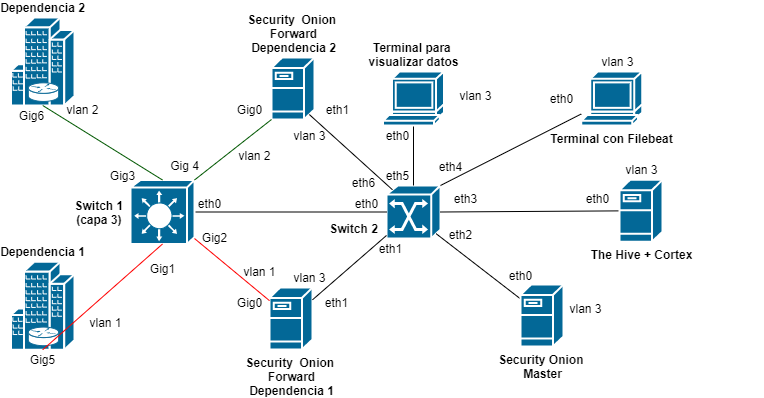
\includegraphics[width=1\textwidth]{./iteracion_2_imagenes/figura_9_topologia_de_prueba_5.png}
        \caption{Topología distribuida con dos nodos Forward}
        \label{fig:iter2_topo_dist}
    \end{figure}

    \end{section}
\label{iteracion2}
